\chapter{Relational Algebra}

\section{Relational Structures}

\subsection{Preliminaries}
\begin{definitionbox}{Schema}
    A description of the database structure.
    \begin{itemize}
        \item {Tables, names and types.
            \begin{minted}{sql}
CREATE TABLE foo (bing INTEGER, zog TEXT, bar INTEGER); 
            \end{minted}
        }
        \item {Integrity constraints (foreign keys, nullability, uniqueness etc)
                \begin{minted}{sql}
ALTER TABLE foo ADD CONSTRAINT foo_key UNIQUE(bing);
                \end{minted}
        }
    \end{itemize}
\end{definitionbox}

Data structures used include:
\begin{center}
    \begin{tabular}{l p{.8\textwidth}}
        Vector & Ordered collection of objects (same type) \\
        Tuple & Ordered collection of objects (can be different types) \\
        Bag & Unordered collection of objects (same type) \\
        Set & Unordered collection of unique objects (same type) \\
    \end{tabular}
\end{center}

\begin{definitionbox}{Relation}
    An array representing an $n$-ary relation $R$ with the properties:
    \\ \begin{minipage}{.49\textwidth}
        \begin{enumerate}
            \setlength\itemsep{0em}
            \item Each row is an $n$-tuple of $R$
            \item Rows are unordered
            \item All rows are unique / distinct
            \item The order of columns corresponds to the ordering of the domains of $R$
            \item Each column is labelled
        \end{enumerate}
        They are almost equivalent to sets tuples (but include labels).
    \end{minipage}
    \hfill
    \begin{minipage}{.5\textwidth}
        \begin{center}
            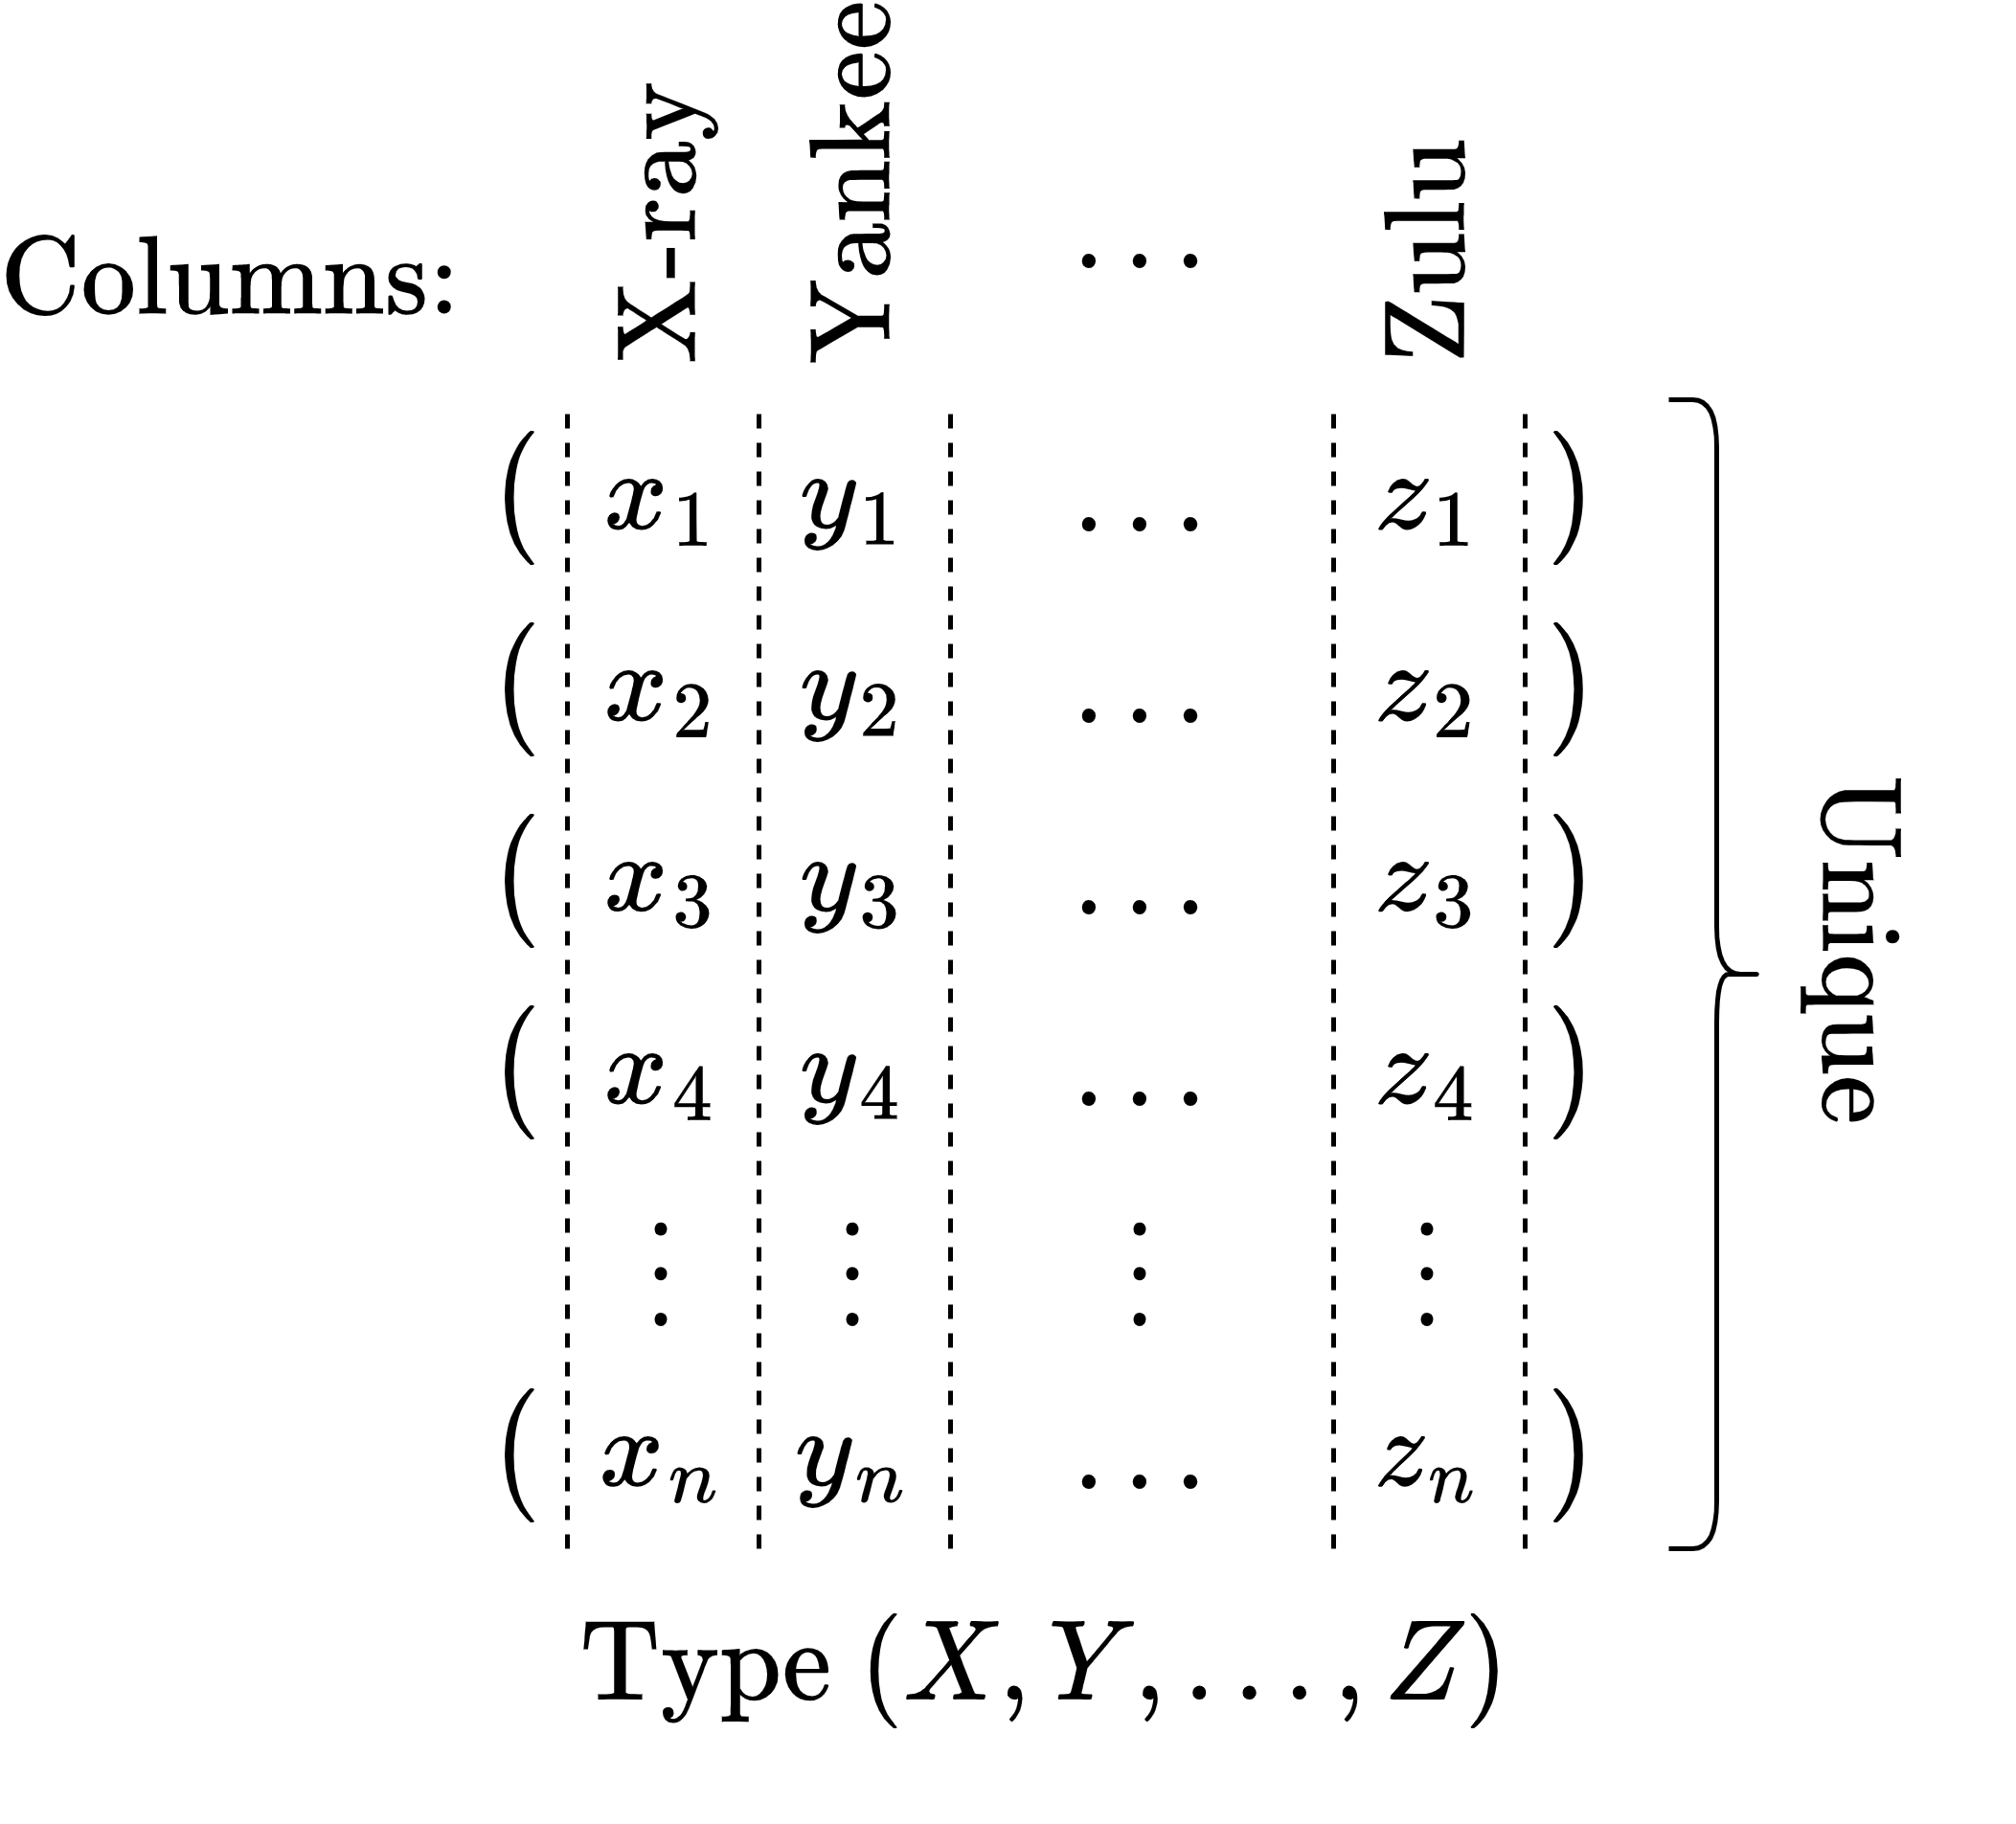
\includegraphics[width=\textwidth]{relational_algebra/images/relation.drawio.png}
        \end{center}
    \end{minipage}
\end{definitionbox}

The minimal set of operators required for the relational algebra are:
\begin{center}
    \begin{tabular}{c c c c c}
        Project & Select & Cross/Cartesian product & Union & Difference \\
    \end{tabular}
\end{center}
Relational algebra is closed:
\begin{itemize}
  \item Every operator outputs a relation
  \item Operators are unary or binary
\end{itemize}

\subsection{Nomenclatures}
\begin{center}
  \begin{tabular}{l p{.8\textwidth}}
    \textbf{Expression} & A composition of operators \\
    \textbf{Logical Plan/Plan} & An expression. \\
    \textbf{Cardinality} & The number of tuples in a set. \\
  \end{tabular}
\end{center}

\section{Implementing Relational Algebra in C++}

In order to implement relations we will make use of several containers from the 
\href{https://en.wikipedia.org/wiki/Standard_Template_Library}{STL (standard template library)}.
\begin{minted}{cpp}
#include <set>
#include <array>
#include <string>
#include <tuple>
#include <variant>

using namespace std;
\end{minted}
We will also make use of \href{https://en.cppreference.com/w/cpp/language/parameter_pack}{\textit{variadict templates}/\textit{parameter packs}} to make our structures not only generic, but generic over $n$ types.
\begin{minted}{cpp}
template<typename... some_types>
\end{minted}
We will also create an operator to inherit from for all operator types:
\begin{minted}{cpp}
template <typename... types> struct Operator : public Relation<types...> {};
\end{minted}

\subsection{Relation}
\begin{minted}{cpp}
template <typename... types> struct Relation {
  // To allow relations to be composed, an output type is required
  using OutputType = tuple<types...>;

  set<tuple<types...>> data;              // table records
  array<string, sizeof...(types)> schema; // column names

  Relation(array<string, sizeof...(types)> schema, set<tuple<types...>> data)
      : schema(schema), data(data) {}
};
\end{minted}

We can hence create a relation using the \mintinline{cpp}{Relation} constructor.
\begin{minted}{cpp}
Relation<string, int, int> rel(
   {"Name", "Age", "Review"},
  {{ "Jim",    33,        3}, 
   { "Jay",    23,        5}, 
   {"Mick",    34,        4}}
);
\end{minted}

\subsection{Project}
\[\Pi_{\underbrace{{a_1, \dots, a_n}}_\text{columns}}(R)\]
A unary operator returning a relation containing only the columns projected ($a_1, \dots, a_n$).
\\
\\ We can first create a projection to 
\begin{minted}{cpp}
template <typename InputOperator, typename... outputTypes>
struct Project : public Operator<outputTypes...> {
  // the single input
  InputOperator input;

  // a variant is a type safe union. It is either a function on rows, or a 
  // mapping of columns 
  variant<function<tuple<outputTypes...>(typename InputOperator::OutputType)>,
          set<pair<string, string>>>
      projections;

  // Constructor for function application
  Project(InputOperator input,
          function<tuple<outputTypes...>(typename InputOperator::OutputType)>
              projections)
      : input(input), projections(projections) {}

  // Constructor for column mapping
  Project(InputOperator input, set<pair<string, string>> projections)
      : input(input), projections(projections) {}
};
\end{minted}

\begin{sidenotebox}{SQL vs RA}
  The default SQL projection does not return a set but rather a multiset / bag. In order to remove duplicates the \mintinline{sql}{DISTINCT} keyword must be used.
\end{sidenotebox}

\subsection{Select}
\[\sigma_{\text{predicate}}(R) \]
Produce a new relation of input tuples satisfying the predicate. Here we narrow this to a condition.

\begin{minted}{cpp}
enum class Comparator { less, lessEqual, equal, greaterEqual, greater };

// user must explicitly set string as a column (less chance of mistake)
struct Column {
  string name;
  Column(string name) : name(name) {}
};

// type alias for comparable values
using Value = variant<string, int, float>;

struct Condition {
  Comparator compare;

  Column leftHandSide;
  variant<Column, Value> rightHandSide;

  Condition(Column leftHandSide, Comparator compare,
            variant<Column, Value> rightHandSide)
      : leftHandSide(leftHandSide), compare(compare),
        rightHandSide(rightHandSide) {}
};
\end{minted}

\begin{sidenotebox}{Enums vs Enum classes}
  \begin{center}
    \begin{tabular}{p{.45\textwidth} p{.45\textwidth}}
      \centerline{\mintinline{cpp}{enum class}} & \centerline{\mintinline{cpp}{enum}} \\
      Enumerations are in the scope of the class & Enumerations are in the same scope as the enum \\
      No implicit conversions. & Implicit conversions to integers. \\ 
    \end{tabular}
  \end{center}
  Enum classes are generally preferred over enums due to the above differences. 
\end{sidenotebox}

\subsection{Cross Product / Cartesian}
\[R_1 \times R_2\]
Creates a new schema concatenating the columns and with the cartesian product of records.

\subsection{Union}

\subsection{Difference}

\subsection{Group Aggregation}

\subsection{Top-N}
\unfinished